\element{inertieeq}{
\begin{question}{jeq 01}
Soit le schéma suivant. Déterminer l'inertie équivalente ramenée à l'arbre moteur 1.
\begin{center}
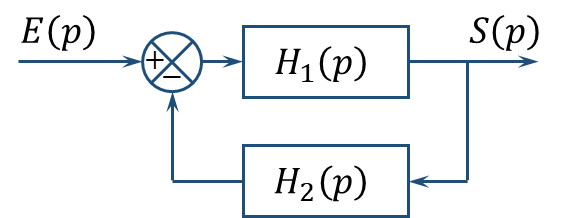
\includegraphics[width=5cm]{fig_01}
\end{center}
\begin{multicols}{2}
	\begin{reponses}
	% 1/2 J_1 \omega_1^2 + 1/2 J_2 \omega_1^2 Z_1^2/Z_2^2 
	\bonne     {$J_1                                  +  \dfrac{Z_1^2}{Z_2^2} J_2$}
	\mauvaise{$\dfrac{Z_2^2}{Z_1^2}J_1 + J_2$}
	\mauvaise{$J_1                                  +  \dfrac{Z_2^2}{Z_1^2} J_2$}
	\mauvaise{$\dfrac{Z_1^2}{Z_2^2}J_1 + J_2  $}
	\end{reponses}
\end{multicols}
\end{question}\\}


\element{inertieeq}{
\begin{question}{jeq 02}
Soit le schéma suivant. Déterminer l'inertie équivalente ramenée à l'arbre 2.
\begin{center}
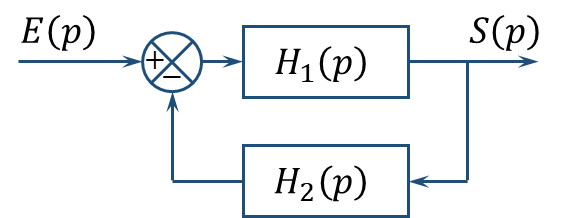
\includegraphics[width=5cm]{fig_01}
\end{center}
\begin{multicols}{2}
	\begin{reponses}
	% 1/2 J_1 \omega_1^2 + 1/2 J_2 \omega_1^2 Z_1^2/Z_2^2 
	\bonne {$\dfrac{Z_2^2}{Z_1^2}J_1 + J_2    $}
	\mauvaise{$J_1 + \dfrac{Z_1^2}{Z_2^2} J_2$}
	\mauvaise{$J_1 + \dfrac{Z_2^2}{Z_1^2}J_2 $}
	\mauvaise{$\dfrac{Z_1^2}{Z_2^2}J_1 + J_2 $}
	\end{reponses}
\end{multicols}
\end{question}\\}


%%%%%%%%%%%%%%%
\element{inertieeq}{
\begin{question}{jeq 03}
Soit le schéma suivant. Déterminer l'inertie équivalente ramenée à l'arbre moteur 1.
\begin{center}
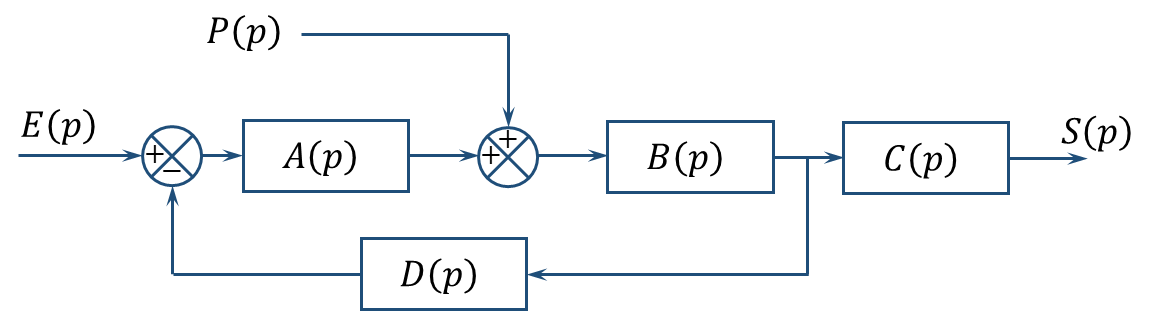
\includegraphics[width=5cm]{fig_02}
\end{center}
\begin{multicols}{2}
	\begin{reponses}
	\bonne     {$ J_1 +  \dfrac{Z_1^2}{Z_2^2} J_2 $}
	\mauvaise{$ \dfrac{Z_2^2}{Z_1^2}J_1 + J_2   $}
	\mauvaise{$ J_1 +  \dfrac{Z_2^2}{Z_1^2} J_2 $}
	\mauvaise{$ \dfrac{Z_1^2}{Z_2^2}J_1 + J_2   $}
	\end{reponses}
\end{multicols}
\end{question}\\}

\element{inertieeq}{
\begin{question}{jeq 04}
Soit le schéma suivant. Déterminer l'inertie équivalente ramenée à l'arbre 2.
\begin{center}
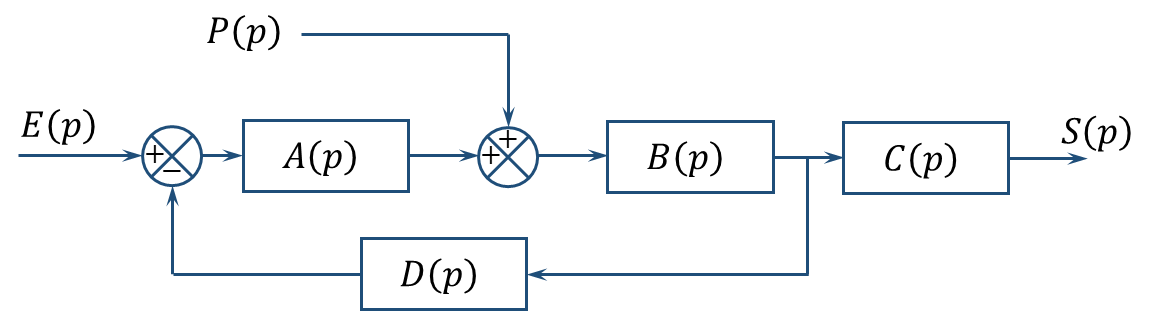
\includegraphics[width=5cm]{fig_02}
\end{center}
\begin{multicols}{2}
	\begin{reponses}
	\bonne     {$ \dfrac{Z_2^2}{Z_1^2}J_1 + J_2 $}
	\mauvaise{$ J_1 + \dfrac{Z_1^2}{Z_2^2} J_2 $}
	\mauvaise{$ J_1 + \dfrac{Z_2^2}{Z_1^2}J_2 $}
	\mauvaise{$ \dfrac{Z_1^2}{Z_2^2}J_1 + J_2 $}
	\end{reponses}
\end{multicols}
\end{question}\\}
%%%%%%%%%%%%

%%%%%%%%%%%%%%%
\element{inertieeq}{
\begin{question}{jeq 05}
Soit le schéma suivant. Déterminer l'inertie équivalente ramenée à l'arbre moteur 1.
\begin{center}
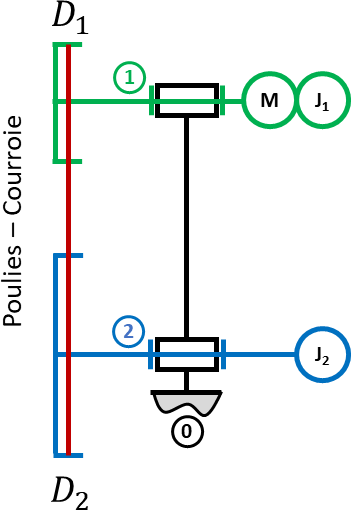
\includegraphics[width=5cm]{fig_03}
\end{center}
\begin{multicols}{2}
	\begin{reponses}
	\bonne     {$ J_1 +  \dfrac{D_1^2}{D_2^2} J_2 $}
	\mauvaise{$  \dfrac{D_2^2}{D_1^2}J_1 + J_2   $}
	\mauvaise{$  J_1 +  \dfrac{D_2^2}{D_1^2} J_2 $}
	\mauvaise{$ \dfrac{D_1^2}{D_2^2}J_1 + J_2   $}
	\end{reponses}
\end{multicols}
\end{question}\\}

\element{inertieeq}{
\begin{question}{jeq 06}
Soit le schéma suivant. Déterminer l'inertie équivalente ramenée à l'arbre 2.
\begin{center}
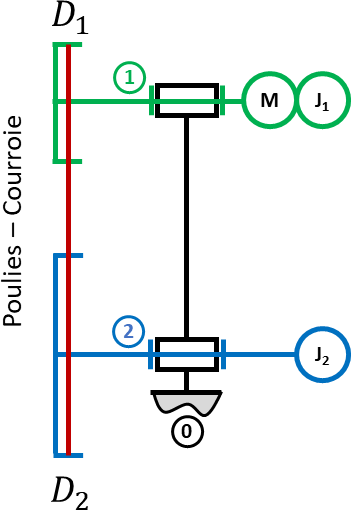
\includegraphics[width=5cm]{fig_03}
\end{center}
\begin{multicols}{2}
	\begin{reponses}
	\bonne     {$ \dfrac{D_2^2}{D_1^2}J_1 + J_2    $}
	\mauvaise{$   J_1 + \dfrac{D_1^2}{D_2^2} J_2  $}
	\mauvaise{$  J_1 + \dfrac{D_2^2}{D_1^2}J_2    $}
	\mauvaise{$  \dfrac{D_1^2}{D_2^2}J_1 + J_2    $}
	\end{reponses}
\end{multicols}
\end{question}\\}
%%%%%%%%%%%%


%%%%%%%%%%%%%%%
\element{inertieeq}{
\begin{question}{jeq 07}
Soit le schéma suivant. Déterminer l'inertie équivalente ramenée à l'arbre moteur 1.
\begin{center}
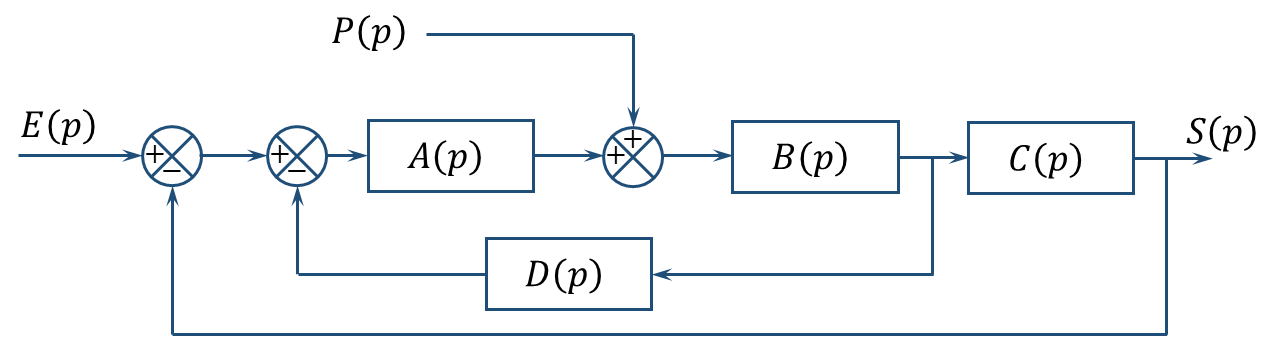
\includegraphics[width=5cm]{fig_04}
\end{center}
% omega_2 = omega_1 \dfrac{D_1}{D_2} 
% v = D3/2 omega_2
% 1/2 (J_1 omega_1^2 + J_2 omega_2^2 + Mv^2)
% 1/2 omega_1^2 (J_1  + J_2  \dfrac{D_1}{D_2}^2 + M (D3/2)^2\dfrac{D_1}{D_2}^2 )

\begin{multicols}{2}
	\begin{reponses}
	\bonne      {$J_1  + J_2  \left(\dfrac{D_1}{D_2}\right)^2 + M \left(\dfrac{D_1D_3}{2D_2}\right)^2$}
	\mauvaise {$J_1 \left(\dfrac{D_2}{D_1}\right)^2 + J_2  + M\left(\dfrac{D_3}{2}\right)^2$}
	\mauvaise {$J_1  + J_2  \left(\dfrac{D_2}{D_1}\right)^2 + M \left(\dfrac{2D_2}{D_1D_3}\right)^2$}
	\mauvaise {$J_1 \left(\dfrac{D_1}{D_2}\right)^2 + J_2  + M \left(\dfrac{D_1D_3}{2D_2}\right)^2$}
	\end{reponses}
\end{multicols}
\end{question}\\}

\element{inertieeq}{
\begin{question}{jeq 08}
Soit le schéma suivant. Déterminer l'inertie équivalente ramenée à l'arbre 2.
\begin{center}
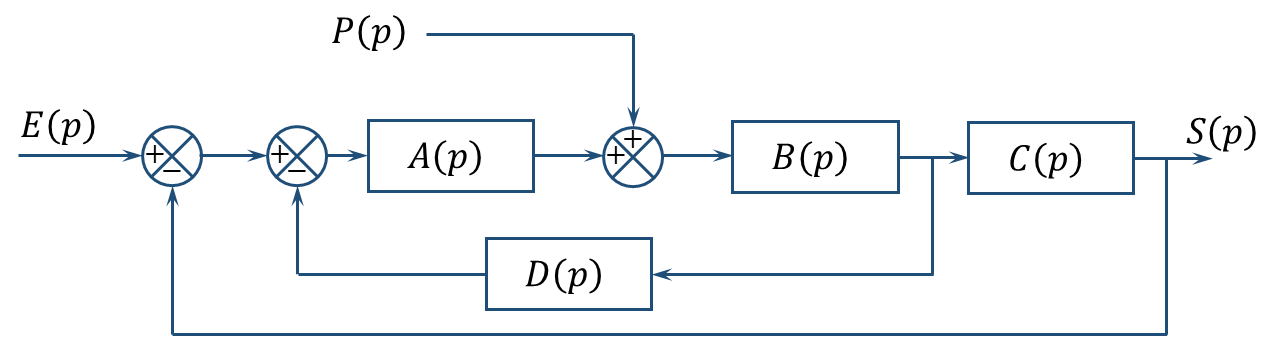
\includegraphics[width=5cm]{fig_04}
\end{center}
% omega_2 = omega_1 \dfrac{D_1}{D_2} 
% v = D3/2 omega_2
% 1/2 (J_1 omega_1^2 + J_2 omega_2^2 + Mv^2)
% 1/2 omega_2^2 (J_1 \left(\dfrac{D_2}{D_1}\right)^2 + J_2  + M\left(\dfrac{D_3}{2}\right)^2)
\begin{multicols}{2}
	\begin{reponses}
	\bonne     {$J_1 \left(\dfrac{D_2}{D_1}\right)^2 + J_2  + M\left(\dfrac{D_3}{2}\right)^2$}
	\mauvaise {$J_1  + J_2  \left(\dfrac{D_1}{D_2}\right)^2 + M \left(\dfrac{D_1D_2}{2D_2}\right)^2$}
	\mauvaise {$J_1  + \left(\dfrac{D_2}{D_1}\right)^2J_2  + M\left(\dfrac{D_3}{2}\right)^2$}
	\mauvaise {$J_1 \left(\dfrac{D_1}{D_2}\right)^2 + J_2  + M\left(\dfrac{D_3}{2}\right)^2$}
	\end{reponses}
\end{multicols}
\end{question}\\}

\element{inertieeq}{
\begin{question}{jeq 09}
Soit le schéma suivant. Déterminer la masse équivalente.
\begin{center}
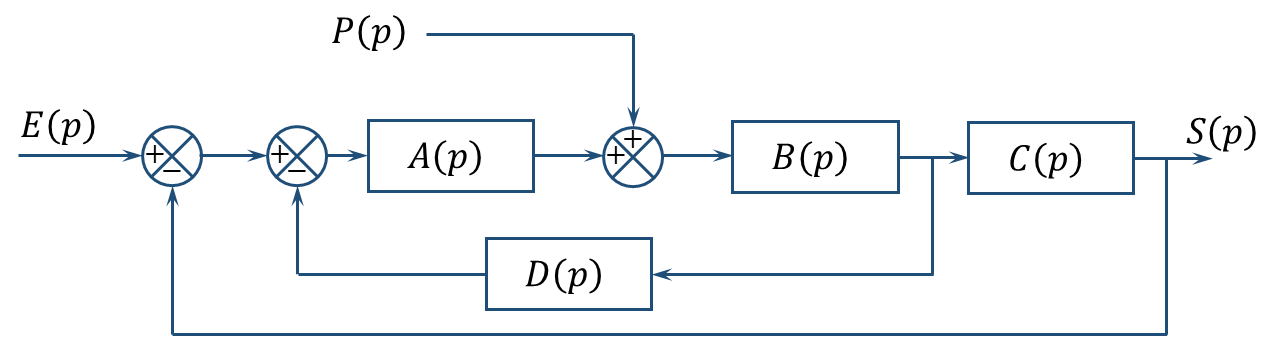
\includegraphics[width=5cm]{fig_04}
\end{center}
% omega_2 = omega_1 \dfrac{D_1}{D_2} 
% v = D3/2 omega_2
% 1/2 (J_1 \dfrac{2D_2}{D_1D_3}^2 + J_2 (2/D3)^2 + Mv^2)
\begin{multicols}{2}
	\begin{reponses}
	\bonne     {$J_1 \left(\dfrac{2D_2}{D_1D_3}\right)^2 + J_2 \left(\dfrac{2}{D3}\right)^2 + M$}
	\mauvaise {$J_1 \left(\dfrac{2}{D3}\right)^2 + J_2 \left(\dfrac{2D_2}{D_1D_3}\right)^2 + M$}
	\mauvaise {$J_1 \left(\dfrac{2D_1}{D_2D_3}\right)^2 + J_2 \left(\dfrac{2}{D3}\right)^2 + M$}
	\mauvaise {$J_1 \left(\dfrac{2D_3}{D_2D_1}\right)^2 + J_2 \left(\dfrac{2}{D3}\right)^2 + M$}
	\end{reponses}
\end{multicols}
\end{question}\\}
%%%%%%%%%%%%


%%%%%%%%%%%%
\element{inertieeq}{
\begin{question}{jeq 10}
On note $v$ la vitesse de la charge $M$ selon la direction horizontale. On note $m$ le module des roues dentées. Exprimer l'inertie équivalente ramenée à l'arbre 1.
% 1/2(   J_1 \omega_1^2 + J_2 \omega_2^2 + Mv^2
%\omega_2 = \omega_1 \dfrac{Z_1}{Z_2}
% v = \dfrac{mZ_2}{2} \omega_2 

%J_1  + J_2 \left(\dfrac{Z_1}{Z_2}\right)^2 + M\left(\dfrac{mZ_2}{2}\dfrac{Z_1}{Z_2}\Right)^2
\begin{center}
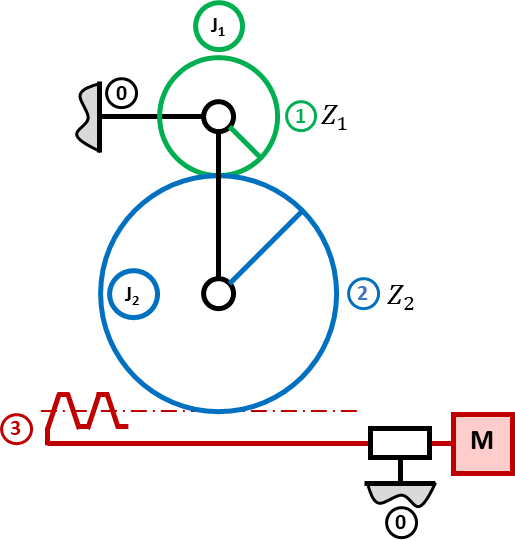
\includegraphics[width=5cm]{fig_05}
\end{center}
\begin{multicols}{2}
	\begin{reponses}	
	\bonne     {$J_1  + J_2 \left(\dfrac{Z_1}{Z_2}\right)^2 + M\left(\dfrac{mZ_1}{2}\right)^2$}
	\mauvaise {$J_1  + J_2 \left(\dfrac{Z_1}{Z_2}\right)^2 + M\left(\dfrac{mZ_2}{2}\right)^2$}
	\mauvaise {$J_1  + J_2 \left(\dfrac{Z_2}{Z_1}\right)^2 + M\left(\dfrac{mZ_1}{2}\right)^2$}		
	\mauvaise {$J_1  + J_2 \left(\dfrac{Z_2}{Z_1}\right)^2 + M\left(\dfrac{mZ_2}{2}\right)^2$}
	\end{reponses}
\end{multicols}
\end{question}\\}

\element{inertieeq}{
\begin{question}{jeq 11}
On note $v$ la vitesse de la charge $M$ selon la direction horizontale. On note $m$ le module des roues dentées. Exprimer l'inertie équivalente ramenée à l'arbre 2.
% 1/2(   J_1 \omega_1^2 + J_2 \omega_2^2 + Mv^2
%\omega_2 = \omega_1 \dfrac{Z_1}{Z_2}
% v = \dfrac{mZ_2}{2} \omega_2 

%J_1\left(\dfrac{Z_2}{Z_1}\right)^2  + J_2 + M \left(\dfrac{mZ_2}{2}\right)^2
\begin{center}
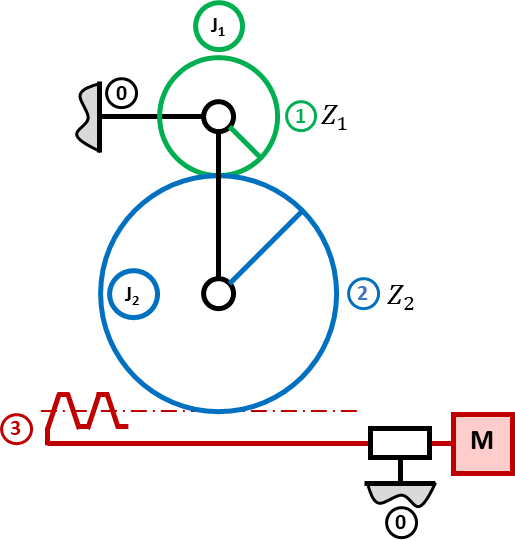
\includegraphics[width=5cm]{fig_05}
\end{center}
\begin{multicols}{2}
	\begin{reponses}	
	\bonne     {$J_1\left(\dfrac{Z_2}{Z_1}\right)^2  + J_2 + M \left(\dfrac{mZ_2}{2}\right)^2$}
	\mauvaise {$J_1\left(\dfrac{Z_1}{Z_2}\right)^2  + J_2 + M \left(\dfrac{mZ_2}{2}\right)^2$}
	\mauvaise {$J_1\left(\dfrac{Z_2}{Z_1}\right)^2  + J_2 + M \left(\dfrac{mZ_1}{2}\right)^2$}		
	\mauvaise {$J_1\left(\dfrac{Z_1}{Z_2}\right)^2  + J_2 + M \left(\dfrac{mZ_1}{2}\right)^2$}
	\end{reponses}
\end{multicols}
\end{question}\\}


\element{inertieeq}{
\begin{question}{jeq 12}
On note $v$ la vitesse de la charge $M$ selon la direction horizontale. On note $m$ le module des roues dentées. Exprimer la masse équivalente.
% 1/2(   J_1 \omega_1^2 + J_2 \omega_2^2 + Mv^2
%\omega_2 = \omega_1 \dfrac{Z_1}{Z_2}
% v = \dfrac{mZ_2}{2} \omega_2 

%J_1\left(\dfrac{2Z_2}{mZ_2 Z_1}\right)^2 + J_2  \left(\dfrac{2}{mZ_2}\right)^2+ M 
\begin{center}
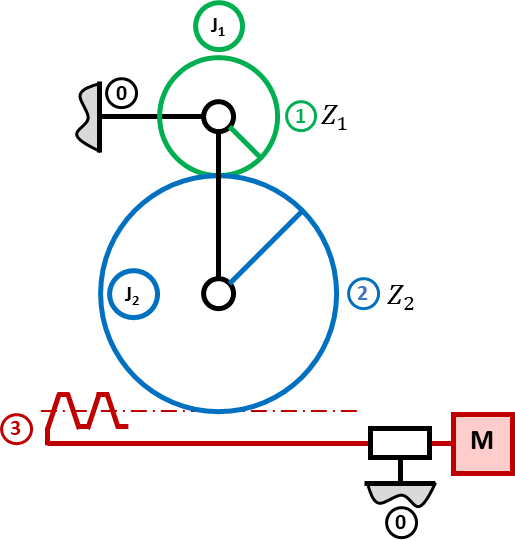
\includegraphics[width=5cm]{fig_05}
\end{center}
\begin{multicols}{2}
	\begin{reponses}	
	\bonne     {$J_1\left(\dfrac{2}{m Z_1}\right)^2 + J_2  \left(\dfrac{2}{mZ_2}\right)^2+ M $}
	\mauvaise {$J_1\left(\dfrac{2}{m Z_1}\right)^2 + J_2  \left(\dfrac{2}{mZ_1}\right)^2+ M $}
	\mauvaise {$J_1\left(\dfrac{2}{m Z_2}\right)^2 + J_2  \left(\dfrac{2}{mZ_2}\right)^2+ M $}		
	\mauvaise {$J_1\left(\dfrac{2}{m Z_2}\right)^2 + J_2  \left(\dfrac{2}{mZ_1}\right)^2+ M $}
	\end{reponses}
\end{multicols}
\end{question}\\}
%%%%%%%%%%%%


%%%%%%%%%%%%%%%%%%%%%%%%
\element{inertieeq}{
\begin{question}{jeq 13}
Soit le schéma suivant. Déterminer l'inertie équivalente ramenée à l'arbre~1.
\begin{center}
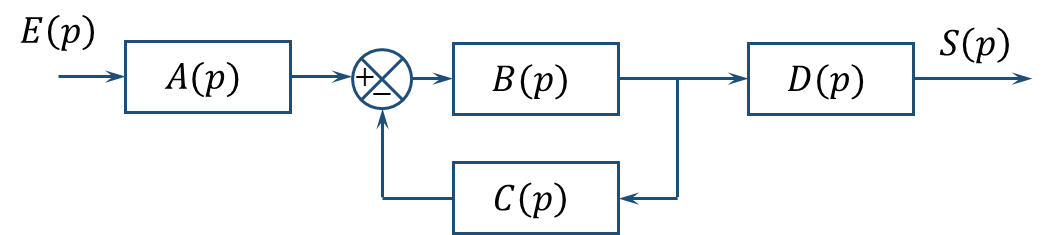
\includegraphics[width=5cm]{fig_06}
\end{center}
% J_1 \omega_1^2 + J_2 \omega_2^2  + J_3 \omega_3^2
%\omega_2 = \omega_1 \dfrac{Z_1}{Z_2}
%\omega_3 = \omega_2 \dfrac{Z_2}{N}

% J_1  + J_2 \left(\dfrac{Z_1}{Z_2}\right)^2  + J_3 \left(\dfrac{Z_1}{Z_2}\dfrac{Z_2}{N}\right)^2
\begin{multicols}{2}
	\begin{reponses}
	\bonne     $J_1  + J_2 \left(\dfrac{Z_1}{Z_2}\right)^2  + J_3 \left(\dfrac{Z_1}{N}\right)^2$	
	\mauvaise $J_1  + J_2 \left(\dfrac{Z_2}{Z_1}\right)^2  + J_3 \left(\dfrac{Z_1}{N}\right)^2$	
	\mauvaise $J_1  + J_2 \left(\dfrac{Z_1}{Z_2}\right)^2  + J_3 \left(\dfrac{Z_2}{N}\right)^2$	
	\mauvaise $J_1  + J_2 \left(\dfrac{Z_2}{Z_1}\right)^2  + J_3 \left(\dfrac{Z_2}{N}\right)^2$	
	\end{reponses}
\end{multicols}
\end{question}\\}


\element{inertieeq}{
\begin{question}{jeq 14}
Soit le schéma suivant. Déterminer l'inertie équivalente ramenée à l'arbre~4.
\begin{center}
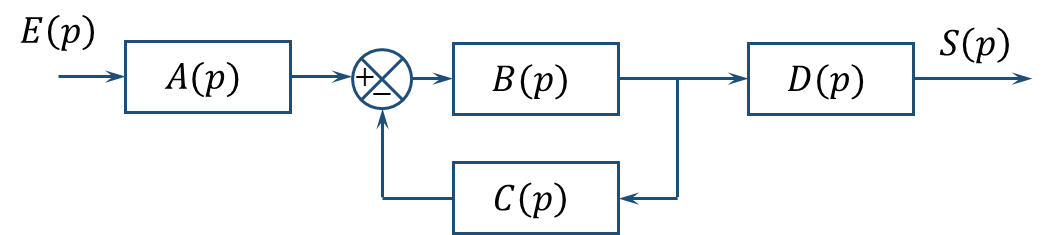
\includegraphics[width=5cm]{fig_06}
\end{center}
% J_1 \omega_1^2 + J_2 \omega_2^2  + J_3 \omega_3^2
%\omega_2 = \omega_1 \dfrac{Z_1}{Z_2}
%\omega_3 = \omega_2 \dfrac{Z_2}{N}

% J_1  + J_2 \left(\dfrac{Z_1}{Z_2}\right)^2  + J_3 \left(\dfrac{Z_1}{Z_2}\dfrac{Z_2}{N}\right)^2
\begin{multicols}{2}
	\begin{reponses}
	\bonne     $J_1\left(\dfrac{Z_2}{Z_1}\right)^2  + J_2   + J_3 \left(\dfrac{Z_2}{N}\right)^2$	
	\mauvaise $J_1\left(\dfrac{Z_2}{Z_1}\right)^2  + J_2   + J_3 \left(\dfrac{Z_2}{N}\right)^2$	
	\mauvaise $J_1\left(\dfrac{Z_1}{Z_2}\right)^2   + J_2  + J_3 \left(\dfrac{Z_1}{N}\right)^2$	
	\mauvaise $J_1\left(\dfrac{Z_1}{Z_2}\right)^2  + J_2   + J_3 \left(\dfrac{Z_1}{N}\right)^2$	
	\end{reponses}
\end{multicols}
\end{question}\\}

\element{inertieeq}{
\begin{question}{jeq 15}
Soit le schéma suivant. Déterminer l'inertie équivalente ramenée à l'arbre~3.
\begin{center}
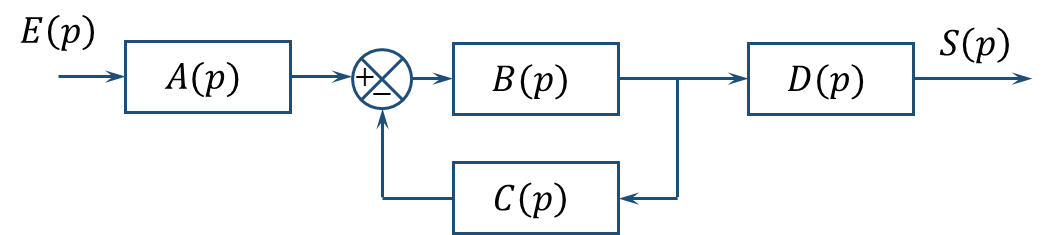
\includegraphics[width=5cm]{fig_06}
\end{center}
% J_1 \omega_1^2 + J_2 \omega_2^2  + J_3 \omega_3^2
%\omega_2 = \omega_1 \dfrac{Z_1}{Z_2}
%\omega_3 = \omega_2 \dfrac{Z_2}{N}

% J_1 \dfrac{Z_1}{Z_2}\dfrac{N}{Z_2}^2 + J_2 \dfrac{N}{Z_2}^2  + J_3 \omega_3^2

\begin{multicols}{2}
	\begin{reponses}
	\bonne      $J_1\left(\dfrac{N}{Z_1}\right)^2  + J_2\left(\dfrac{N}{Z_2}\right)^2   + J_3 $	
	\mauvaise $J_1\left(\dfrac{N}{Z_2}\right)^2  + J_2\left(\dfrac{N}{Z_2}\right)^2   + J_3 $	
	\mauvaise $J_1\left(\dfrac{N}{Z_1}\right)^2  + J_2\left(\dfrac{N}{Z_1}\right)^2   + J_3 $	
	\mauvaise $J_1\left(\dfrac{Z_1}{N}\right)^2  + J_2\left(\dfrac{Z_2}{N}\right)^2   + J_3 $	
	\end{reponses}
\end{multicols}
\end{question}\\}


%%%%%%%%%%%%%%%%%%%
%\element{inertieeq}{
%\begin{question}{jeq 10}
%On note $v$ la vitesse de la charge $M$ selon la direction horizontale. Exprimer $v$ en fonction de 
%$\omega_{10}$ (en valeur absolue). On note $p$ le pas de la vis.
%\begin{center}
%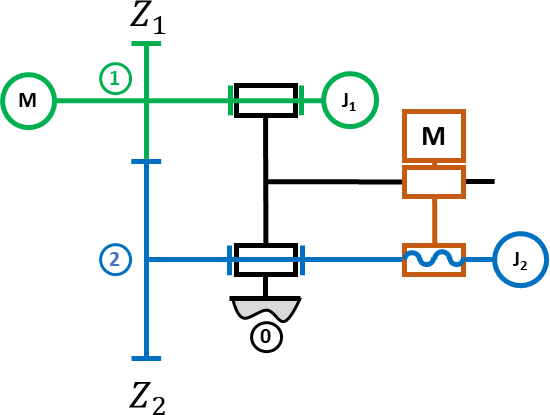
\includegraphics[width=5cm]{fig_07}
%\end{center}
%\begin{multicols}{4}
%	\begin{reponses}	
%	\mauvaise{$v = \dfrac{ Z_2  }{ Z_1  p } \omega_{10}$}
%	\mauvaise{$v = \dfrac{Z_2 p}{2 Z_1  \pi } \omega_{10}$}
%	\mauvaise{$v = \dfrac{2 Z_1 \pi }{ Z_2  p } \omega_{10}$}
%	\bonne{$v = \dfrac{Z_1 p}{2 Z_2  \pi } \omega_{10}$}
%	\end{reponses}
%\end{multicols}
%\end{question}\\}
%
